%
% File ACL2016.tex
%

\documentclass[11pt]{article}
\usepackage{acl2016}
\usepackage{times}
\usepackage{latexsym}
\usepackage{url}
\usepackage{booktabs}
\usepackage{graphicx}
\usepackage{color}
\usepackage{amsmath}
\aclfinalcopy 

\usepackage[authoryear]{natbib}
\usepackage{url}

\title{The Linguistic Evolution of AI and ML in English Literature}
\author{Mohamed Liban S5371120\\
Length: 3-4 pages}
\date{16-01-2024}


\begin{document}
\maketitle 

%%% YOUR PART HERE
\begin{abstract}
{The purpose of this study is to examine how the terms artificial intelligence (AI) and machine learning (ML) have changed linguistically over the last seven decades in English literature. The English Google Ngram Books Viewer dataset is used in the study to examine trends in the terms' evolution and their relationship to technological advancements. This research helps in understanding language dynamics in connection to emerging technologies.}
\end{abstract}

%% IMPORTANT: KEEP ALL SECTIONS (headers)
%% remove the 'red' text parts

\section{Introduction}

{The use of words related to AI and ML has certainly been impacted by the quick development of the technology related to them. The purpose of this study is to examine which process the linguistic shifts in the last 70 years increased in relation to the use of AI and ML terms in English literature. We hypothesize that linguistic shifts in these terms reflect the gradual nature of technological progress, which recently saw significant advancements in the late 2010s. Here are the variables that were used:
}
{


\begin{itemize}
    \item[\textbullet] Independent Variables:
    \begin{itemize}
        \item Time Period: The years that are being investigated, including significant eras of technological development.
        \item AI Frequency (\%): The proportionate frequency, within the given time period, of the term "artificial intelligence" in English literature.
        \item ML Frequency (\%): The proportion of times the term "machine learning" appeared in English literature over the course of the given time frame.
    \end{itemize}
    \item[\textbullet] Dependent Variable(s):
    \begin{itemize}
        \item Language Shift in AI and ML Terms: This is a reference to the noted changes in the frequency of occurrences of the terms "AI" and "ML" in English literature over time. The dependent variable captures changes in language use, which is a sign of how technology is evolving.
    \end{itemize}
\end{itemize}



\section{Related Work}



For this research, we looked at articles and papers that explored the history and evolution of  artificial intelligence (AI) and machine learning (ML) over the past 70 years.

\citep{Feigenbaum:ea:1980}'s seminal work in 1980 provides insights into the early landscape of expert systems.
The study by \citep{Washington:2006} critically reviews the history of AI, including the AI Winter in the 1990s
Lastly, the study by \cite{PET:2021} contains the most recent history in terms of artificial intelligence (AI) and machine learning (ML).

The results of the current study support this renewed focus, and the articles provide a wealth of relevant information. They also correspond with the linguistic shifts in AI and ML terms that have been observed in English literature.

\section{Data}

The English Google Ngram Books dataset is used as a representative source for English literature in order to carry out this research. The frequencies of "AI" and "ML," expressed as percentages over various time periods, are presented as the independent variables. The dataset covers the years 1950 to 2019 and highlights big developments in ML and AI during that time. The current decade should ideally be covered, but Google Ngram Books Viewer only extends to 2019.

\begin{table}[hbtp]\centering
\begin{tabular}{|ccc|}
\hline
Time Period & AI Freq (\%) & AI Freq (\%)\\
\hline
1950 & X & X\\
1970 & X & X\\
1990 & X & X\\
2010 & X & X\\
2019 & X & X\\

\hline
\end{tabular}
\caption{X stands for the value of frequency in \%}
\label{tbl:results}
\end{table}

\vspace{5pt}

\paragraph{Data collection} We accessed the English dataset for English literature through Google Ngram Books. We also used the Google search engine to look for the years of all major technological advancements. We made sure to start from 1950 to also capture the earlier advancements in technology in terms of AI and ML. After capturing the data, we tried to connect a peak of the graph to (the year of) an invention or major technological resurgence.


\paragraph{Pre-processing} To make sure that the raw frequency data was accurate, very little pre-processing was done. We only used case-insensitivity and a smoothing of 0 to ensure that we get the most realistic raw data in terms of the graph.



\section{Predicted Results}

Based on the findings of the literature review, we think that the projected result will indicate a noticeable increase in the occurrence of AI and ML terms in English literature during the investigated period.

Table~\ref{tbl:results} 


\begin{table}[hbtp]\centering
\begin{tabular}{|ccc|}
\hline
Time Period & AI Freq (\%) & AI Freq (\%)\\
\hline
1950 & 0.0005\% & 0.0003\%\\
1970 & 0.0008\% & 0.0005\%\\
1990 & 0.0013\% & 0.0009\%\\
2010 & 0.0019\% & 0.0011\%\\
2019 & 0.0029\% & 0.0021\%\\

\hline
\end{tabular}
\caption{Predicted results in \%}
\label{tbl:results}
\end{table}

\section{Results} 

Based on our actual research, we noticed that the rise of the graphs was not as gradual as we initially thought. Rather, it had a massive upsurge starting in the 1980s all the way to its peak in 1988. After which, it had a massive decline until the early 2000s. From 2015 onwards, it has only been rising, with 2019 being the all-time high in the investigated period.

\begin{table}[hbtp]\centering
\begin{tabular}{|ccc|}
\hline
Time Period & AI Freq (\%) & AI Freq (\%)\\
\hline
1950 & 0.0000007824\% & 0.0000000882\%\\
1970 & 0.0000372525\% & 0.0000040364\%\\
1990 & 0.0006112526\% & 0.0000658826\%\\
2010 & 0.0002292496\% & 0.0001457044\%\\
2019 & 0.0005921173\% & 0.0008143430\%\\

\hline
\end{tabular}
\caption{Results in \%}
\label{tbl:results}
\end{table}

\begin{figure}
  \centering
  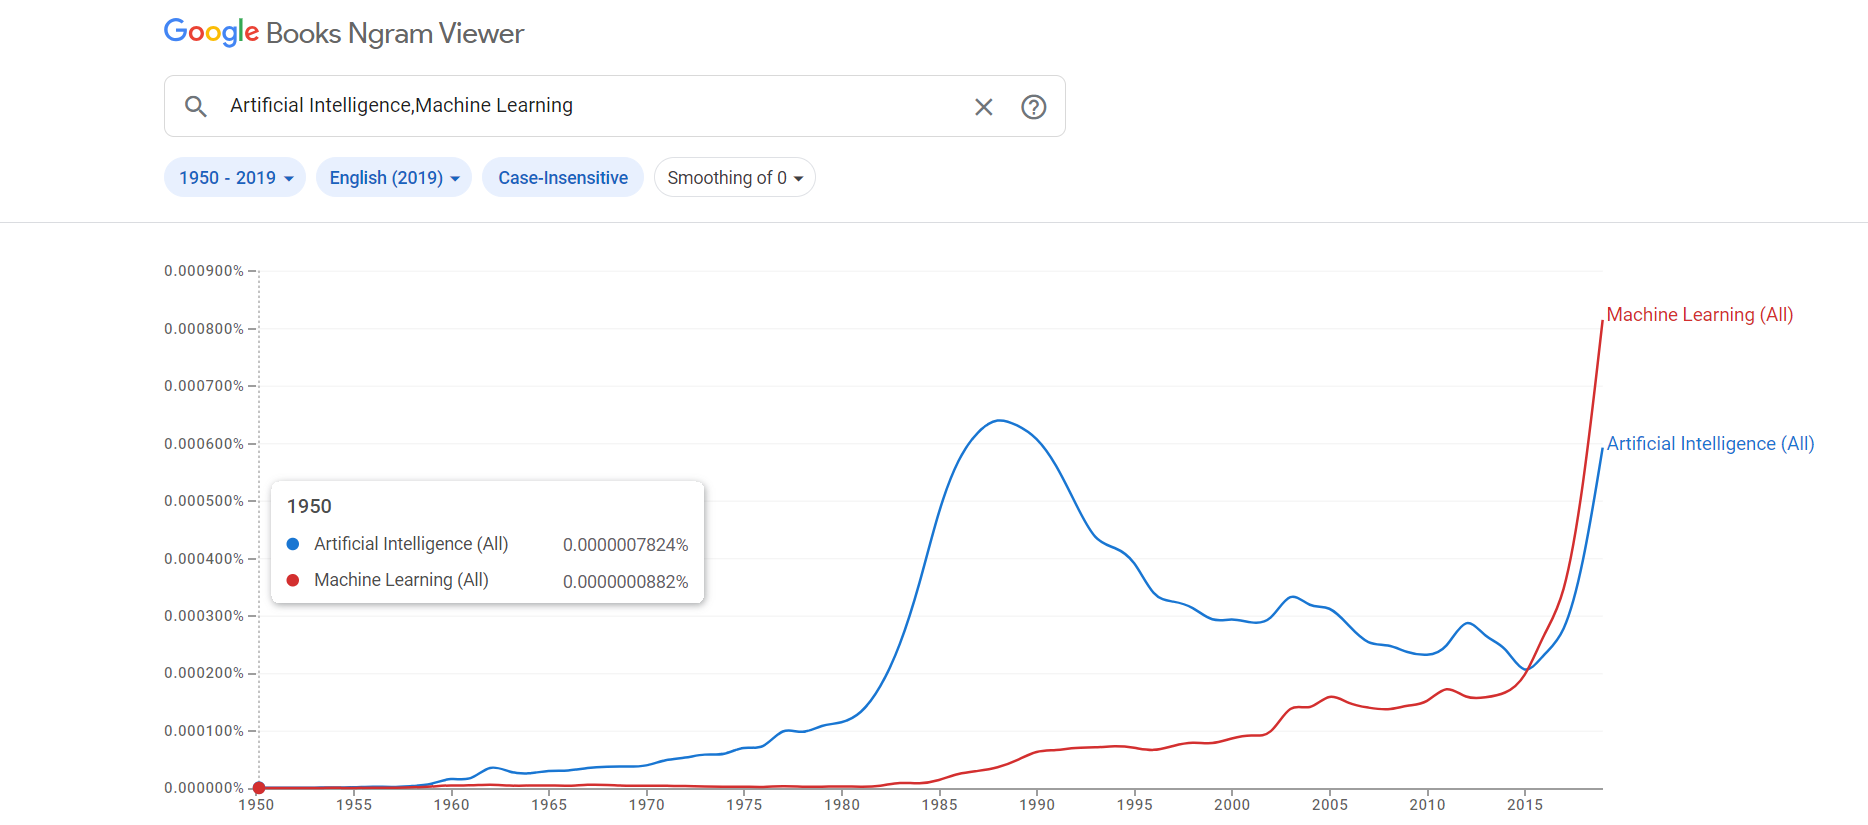
\includegraphics[width=0.45\textwidth]{Screenshot 2024-01-13 210601.png}
  \caption{"Artificial Intelligence" and "Machine Learning" in 1950}
  \label{fig:ngram1}
\end{figure}

\begin{figure}
  \centering
  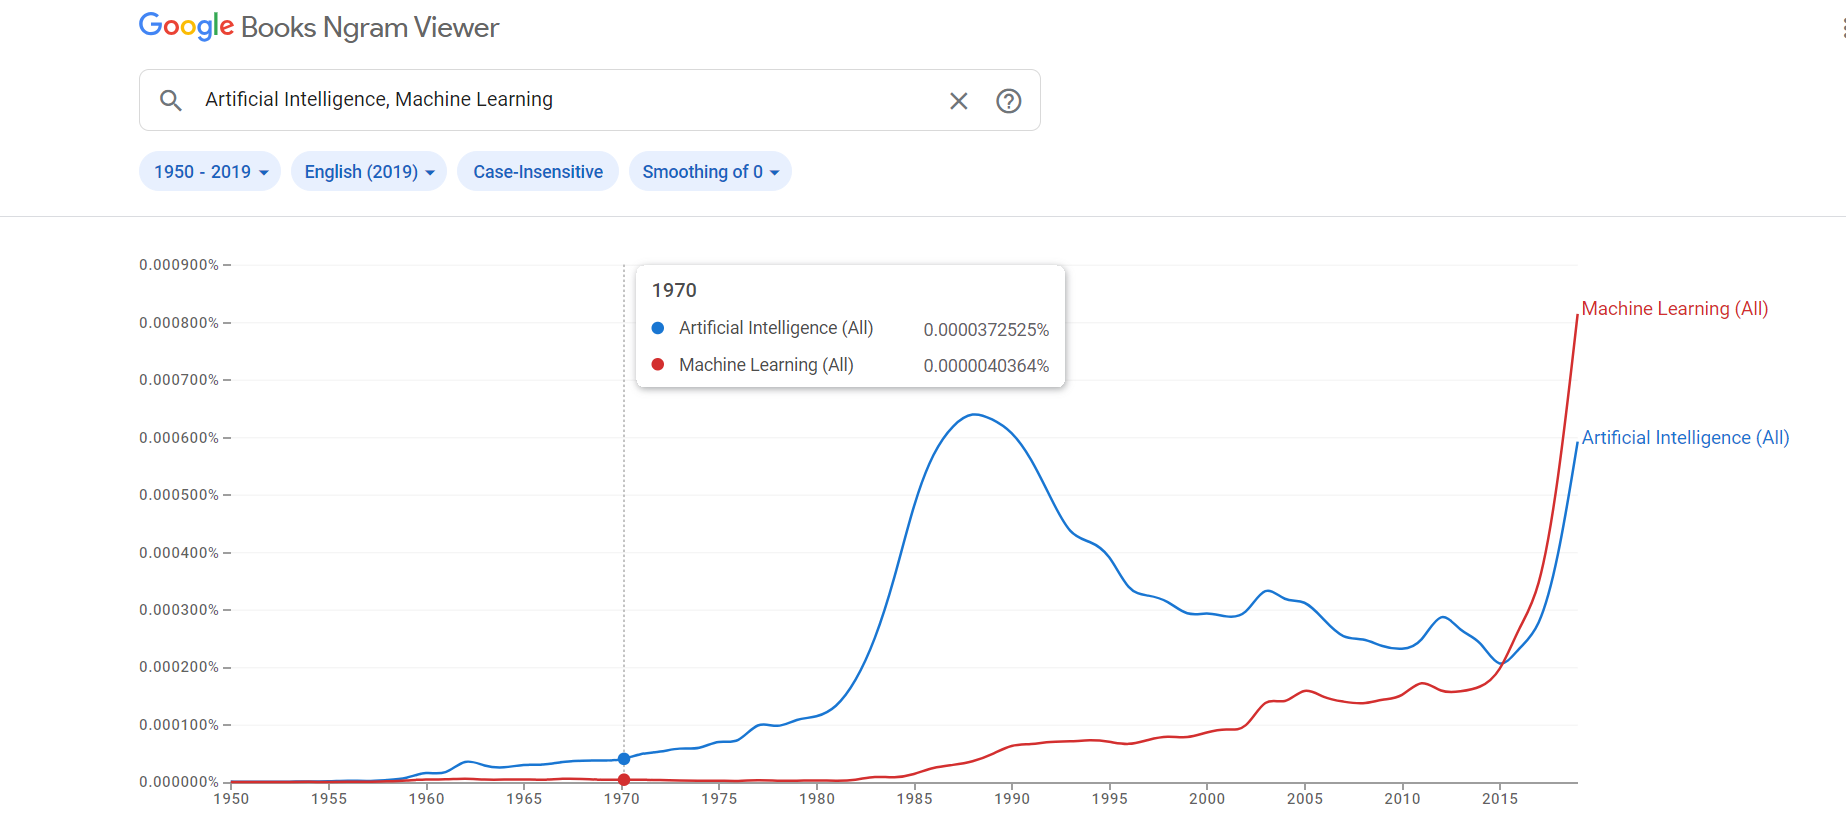
\includegraphics[width=0.45\textwidth]{Screenshot 2024-01-16 214359.png}
  \caption{"Artificial Intelligence" and "Machine Learning" in 1970}
  \label{fig:ngram1}
\end{figure}

\paragraph{}The sudden rise from the start of the 1980s had to do with the investing and funding of governments and organizations and the use of expert systems, which are "intelligent computer program that uses knowledge and inference
procedures" according to \cite{Feigenbaum:ea:1980}. \citep{Washington:2006} states that, by the end of the 1980s, more than half of Fortune 500 companies were creating or maintaining expert systems. \cite{Washington:2006} claims that the application of expert systems grew 30\% annually.

\begin{figure}
  \centering
  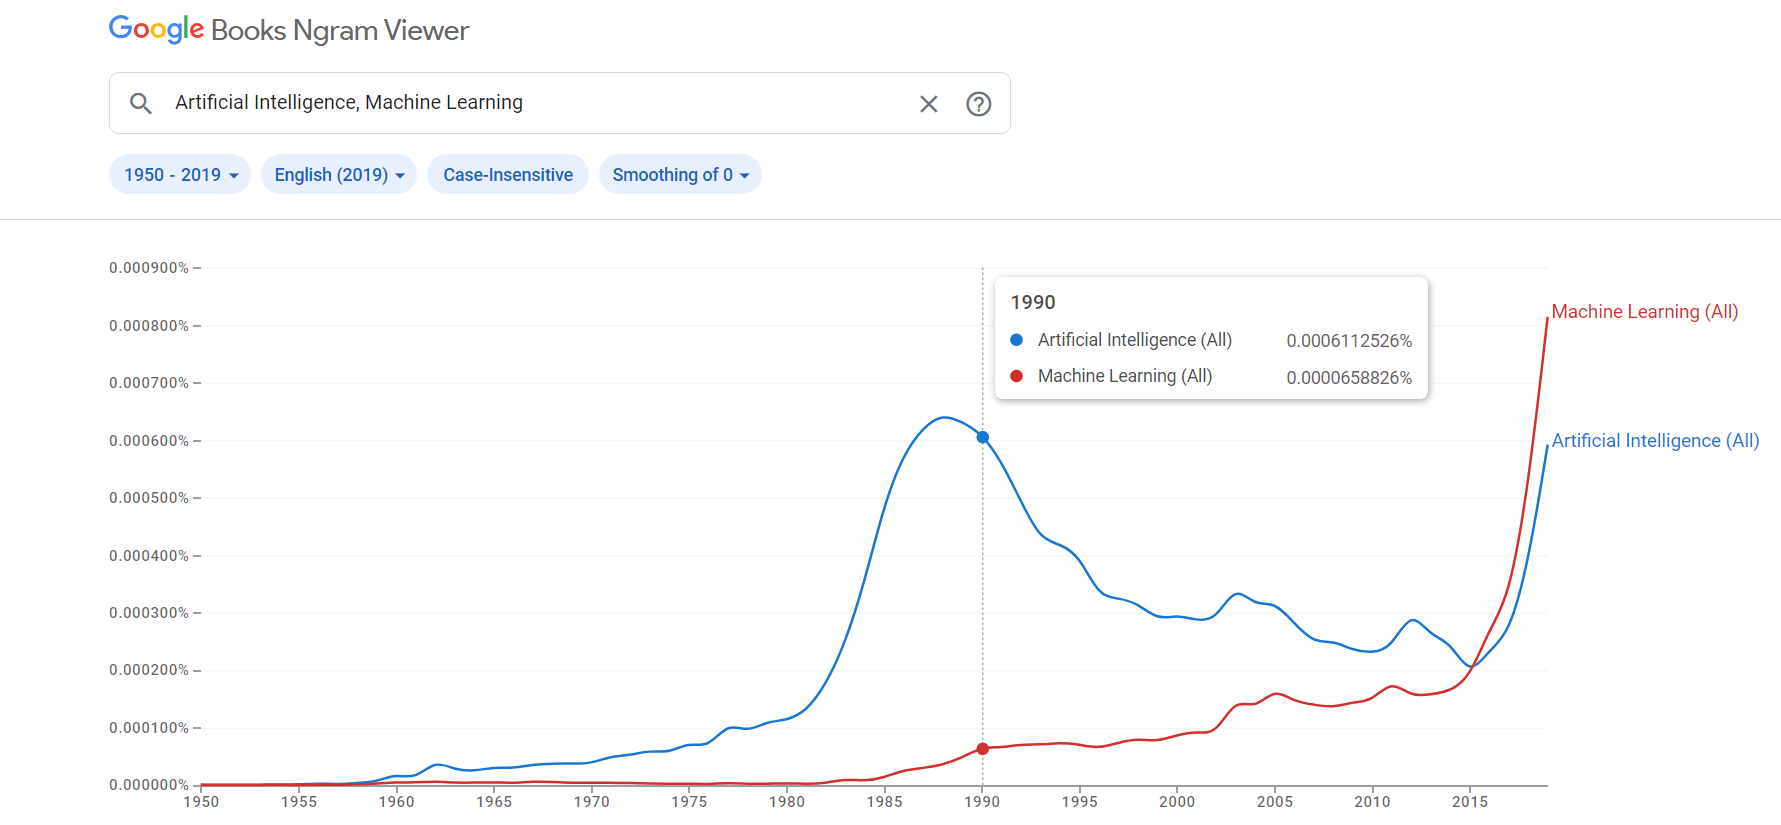
\includegraphics[width=0.45\textwidth]{Screenshot 2024-01-16 214434.png}
  \caption{"Artificial Intelligence" and "Machine Learning" in 1990}
  \label{fig:ngram1}
\end{figure}

The strong decline from the rise had to do with the AI Winter in the 1990s. It was caused by incredibly high expectations, which were impossible to fulfill. According to \citep{PET:2021}, the specialized requirements of expert systems proved too much for hardware manufacturers to handle. \cite{PET:2021} stated that the AI Winter "had been so harsh that AI researchers subsequently tended to avoid even the term “AI” by choosing other titles such as “informatics” or "analytics”."

\begin{figure}
  \centering
  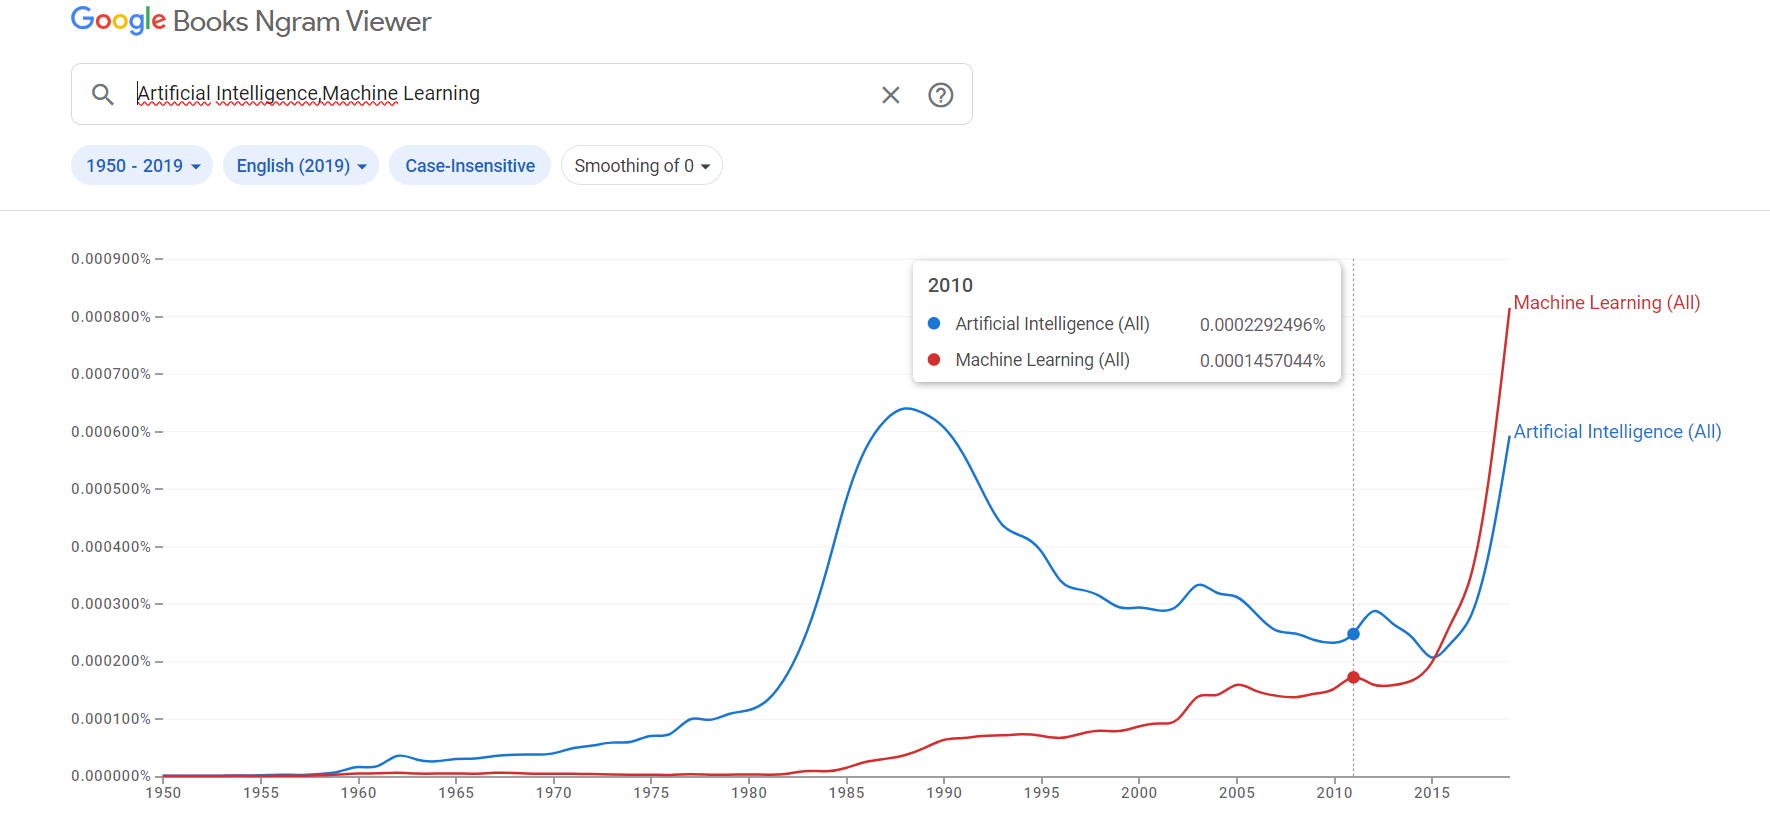
\includegraphics[width=0.45\textwidth]{Screenshot 2024-01-16 220127.png}
  \caption{"Artificial Intelligence" and "Machine Learning" in 2010}
  \label{fig:ngram1}
\end{figure}

The current rise from 2015 onwards has to do with the breakthroughs of deep learning and AI entering businesses and industries. \cite{PET:2021} states, "from 2010 to 2020, global investment in AI-based startup companies has steadily grown from \$1.3B to more than \$40B, with an average annual growth rate of nearly 50\%"

\begin{figure}
  \centering
  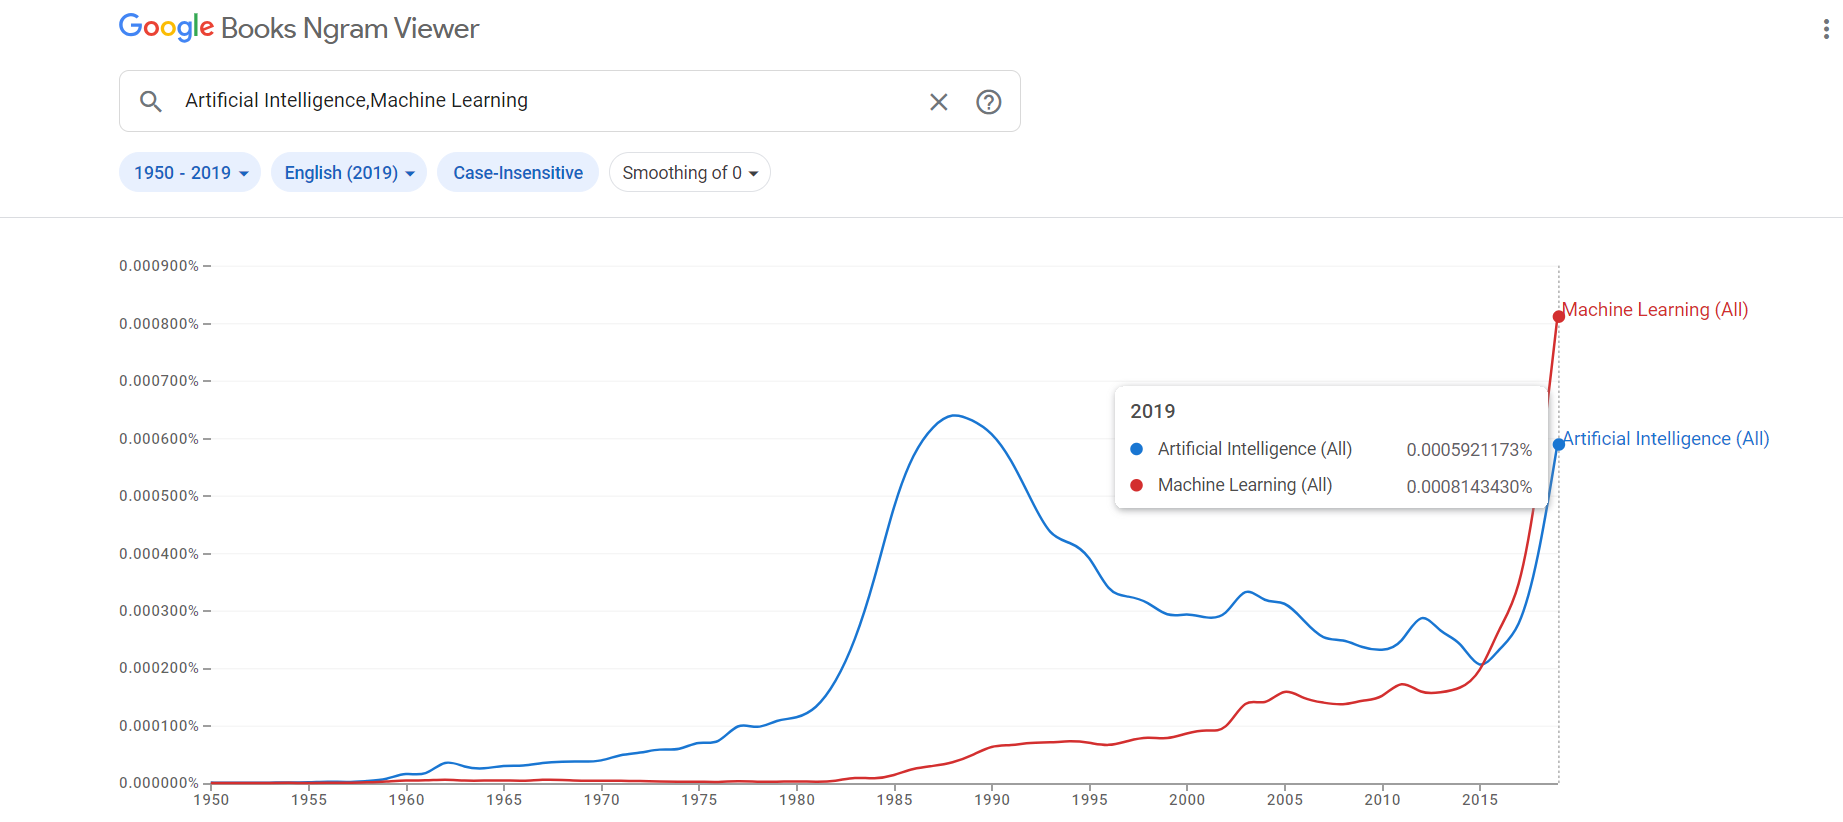
\includegraphics[width=0.45\textwidth]{Screenshot 2024-01-13 211035.png}
  \caption{"Artificial Intelligence" and "Machine Learning" in 2019}
  \label{fig:ngram1}
\end{figure}

\paragraph{Discussion}
We did not initially expect the graph to have such a spike in the previous century. However, we learned that people in the 80s and earlier were already aware of AI and it's implications. This is also obvious when one also thinks about the desires of industries to automate and optimize production. We have learned much with regards to the history of AI; it's good times and it's bad times. Overall, one can say that the rise (and fall) of AI and ML was most definitely not gradual.

\section{Conclusion}

In conclusion, our research examined linguistic changes in English literature pertaining to the terms "machine learning" (ML) and "artificial intelligence" (AI) over a seven-decade period. The graphs revealed, against our initial prediction, a notable increase in the 1980s, a decrease in the 1990s (AI Winter), and a resurgence since 2015. This pattern shows how language use has been impacted by past events like government investments and the AI Winter. The recent increase is consistent with deep learning breakthroughs and greater AI integration. The dynamic relationship between language and technological evolution in literature is highlighted by our findings.



\bibliographystyle{chicago}
\bibliography{mybib.bib}

\end{document}



